

\documentclass[11pt]{amsart}

\usepackage{amsfonts,amsmath,amssymb,amsthm,enumerate}
\usepackage[latin1]{inputenc}
\usepackage{hyperref}
\usepackage{tikz}
\usetikzlibrary{calc}
\usepackage[all]{xy}
\usepackage{float}

 

 
 
 
 
 
 
 
 
 

{\theoremstyle{plain}
\newtheorem{theorem}{Theorem}    
\newtheorem*{theorem*}{Theorem}
\newtheorem*{theorem1}{Theorem 1}
\newtheorem*{theoremB}{Theorem B}
\newtheorem{lemma}[theorem]{Lemma}       
\newtheorem{proposition}[theorem]{Proposition}      
\newtheorem{proposition*}{Proposition} 
\newtheorem{corollary}[theorem]{Corollary}      
\newtheorem{conjecture}[theorem]{Conjecture}
\newtheorem{definition}[theorem]{Definition}      
}
{\theoremstyle{remark}

\newtheorem*{remark*}{Remark}  
\newtheorem{remark}[theorem]{Remark}   
\newtheorem{example}[theorem]{Example}
\newtheorem{question}{Question}
\newtheorem*{question*}{Question}
}

\setlength{\parindent}{0pt}
\floatplacement{figure}{H}
 
\title{The braid group of a necklace}

\date{\today}

\author{Paolo Bellingeri}
\email{Paolo.Bellingeri@unicaen.fr}

\author{Arnaud Bodin}
\email{Arnaud.Bodin@math.univ-lille1.fr}

\address{Laboratoire Nicolas Oresme,
 Universit\'e de Caen, 14032 Caen, France}  

\address{Laboratoire Paul Painlev\'e, Math\'ematiques, Universit\'e 
Lille 1, 59655 Villeneuve d'Ascq, France}

\subjclass[2010]{20F36 (20F65, 57M25)}

\keywords{Configuration space; Braid group; Automorphism; Knots and links}

\begin{document}

\begin{abstract}
We show several geometric and algebraic aspects of a \emph{necklace}:
a link composed with a core circle and a series of circles linked to this core.
We first prove that the fundamental group of the configuration space of necklaces 
(that we will call  braid group of a necklace) is 
isomorphic to  the braid group over an annulus quotiented by the square of the center.
We then define   braid groups of necklaces and  affine braid groups of type $\mathcal{A}$
in terms  of  automorphisms of  free groups and characterize these automorphisms 
among all automorphisms of free groups.  In the case of affine braid groups of type $\mathcal{A}$
such representation is faithful.
\end{abstract}

\maketitle

\section{Introduction}

The braid group $B_n$ can be defined as the fundamental group of the configuration space  
of $n$ distinct points on a disk.
By extension, when we replace the disk by another surface $\Sigma$, we define the \emph{braid group on $n$ strands over $\Sigma$}
as the fundamental group of the configuration space of $n$ distinct points on $\Sigma$.
A particular case is when $\Sigma$ is the annulus: the braid group of the annulus,
denoted by $CB_n$ (for \emph{circular braid group}) is the fundamental group of the configuration 
space $\mathcal{CB}_n$ of $n$ distinct points over an annulus.
\begin{figure}
 
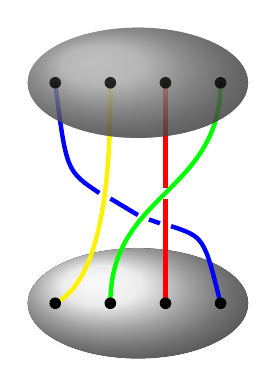
\begin{tikzpicture}[scale=0.7]
\fill [ball color=gray!20] (0,0) ellipse (2 and 1);

\draw[ultra thick,yellow] (-1.5,0) .. controls (-0.5,0.5)  and (-0.5,3) .. (-0.5,4);

\draw[ultra thick,green] (-0.5,0) .. controls (-0.5,2)  and (1.5,2) .. (1.5,4);

\draw[ultra thick,red] (0.5,0)--(0.5,1.9);
\draw[ultra thick,red] (0.5,2.1)--(0.5,4);

\draw[ultra thick,blue] (1.5,0) .. controls (1.2,1.2)   ..(0.6,1.4);
\draw[ultra thick,blue] (0.4,1.45)--(0.2,1.52);
\draw[ultra thick,blue] (0,1.6)--(-0.5,1.9);
\draw[ultra thick,blue] (-0.7,2).. controls (-1.3,2.4)   ..(-1.5,4);

\fill [ball color=gray!20,opacity=0.6] (0,4) ellipse (2 and 1);

\foreach \i in{-1.5,-0.5,0.5,1.5}{
  \fill[black,opacity=1]({\i},0) circle(3pt);
  \fill[black,opacity=0.8]({\i},4) circle(3pt);
};

\end{tikzpicture}
 \qquad
 
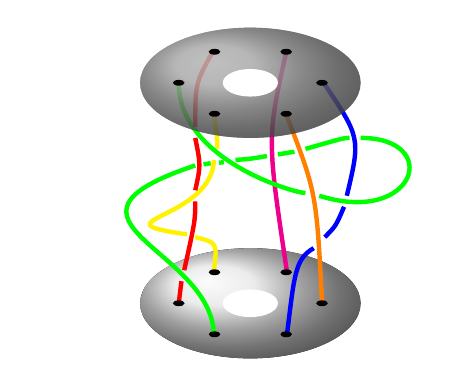
\begin{tikzpicture}[scale=0.7]
\fill [ball color=gray!20] (0,0) ellipse (2 and 1);
\fill [white] (0,0) ellipse (0.5 and 0.25);

\draw[ultra thick,orange] (0:1.3)  .. controls (1.2,2).. (0.66,3.4);

\draw[ultra thick,blue] (0.66,-0.6).. controls (0.8,0.5)  and (0.8,0.8) ..(1.15,1);
\draw[ultra thick,blue] (1.35,1.20).. controls (1.55,1.4)..(1.7,1.75);
\draw[ultra thick,blue] (1.75,1.95).. controls (2,3)   ..(1.33,4);

\draw[ultra thick,magenta] (0.66,0.6) .. controls (0.3,3)  .. (0.66,4.6);

\draw[ultra thick,yellow] (-0.66,0.6) .. controls (-0.6,1.1)  .. (-1,1.2);
\draw[ultra thick,yellow] (-1.15,1.25) .. controls (-2.9,1.5) and (-0.7,1.5) .. (-0.66,2.6);
\draw[ultra thick,yellow] (-0.6,2.8) .. controls (-0.6,3)  .. (-0.66,3.4);

\draw[ultra thick,green] (-0.66,-0.6) .. controls (-0.66,1)  and (-4,1.5)  .. (-1,2.5);
\draw[ultra thick,green] (-0.85,2.52) -- (-0.72,2.54);
\draw[ultra thick,green] (-0.57,2.55) --(-0.48,2.56);
\draw[ultra thick,green] (-0.27,2.6).. controls (0,2.62) .. (0.3,2.67);
\draw[ultra thick,green] (0.5,2.7) -- (0.8,2.75);
\draw[ultra thick,green] (1,2.8) .. controls (1.7,3) .. (1.8,3);
\draw[ultra thick,green] (2,3) .. controls (3.5,3) and (3,1.4) .. (1.25,1.95);
\draw[ultra thick,green] (1,2) .. controls (0.8,2)  and (-1.3,2.6)  .. (-1.3,4);

\draw[ultra thick,red] (-1.3,0) -- (-1.25,0.4);
\draw[ultra thick,red] (-1.2,0.6) .. controls (-1,1.5) .. (-1,1.85);
\draw[ultra thick,red] (-1,2.05) .. controls (-0.9,2.5) .. (-1,3);
\draw[ultra thick,red] (-1,3.2) .. controls (-1,4)  .. (-0.66,4.6);

\fill [ball color=gray!20,opacity=0.6] (0,4) ellipse (2 and 1);
\fill [white] (0,4) ellipse (0.5 and 0.25);

\begin{scope}[yscale=0.5]
\foreach \i in{0,60,...,300}{
  \fill[black,opacity=1]({\i}:1.3) circle(3pt);
  \fill[black,opacity=1] (0,8)+({\i}:1.3) circle(3pt);
};
\end{scope}

\end{tikzpicture}

 \caption{A braid with $4$ strands over a disk (left). 
 A braid with $6$ strands over an annulus (right).}
\end{figure}

There is a 3-dimensional analogous of $B_n$: it is the fundamental group of all configurations of $n$
unlinked Euclidean circles. Following  \cite{BH} we will denote by $\mathcal{R}_n$ the space of configurations of $n$
unlinked Euclidean circles and by $R_n$ its fundamental group (called \emph{group of rings} in \cite{BH}).
The group $R_n$  is generated by $3$ types of moves (see figure \ref{fig:moves}).
\begin{figure}
 
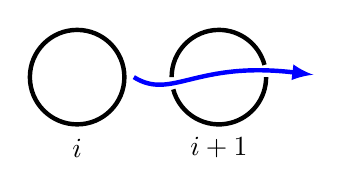
\begin{tikzpicture}[scale=0.6]

 \draw[ultra thick]  (0:1) arc (0:360:1);

\begin{scope}[xshift=3cm]
  \draw[ultra thick]  (-165:1) arc (-165:0:1);
  \draw[ultra thick]  (-180:1) arc (-180:-345:1);
\end{scope}

\draw[->,>=latex,ultra thick,blue] (1.2,0.) .. controls (2,-0.5)  and (2.5,0.35) .. (5,0.05);

 \node at (0,-1.5) {$i$}; 
 \node at (3,-1.5) {$i+1$}; 
\end{tikzpicture}
 \qquad
 
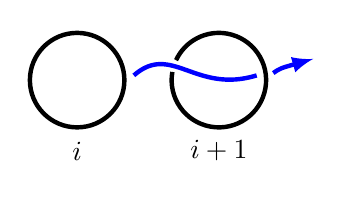
\begin{tikzpicture}[scale=0.6]

 \draw[ultra thick]  (0:1) arc (0:360:1);

\begin{scope}[xshift=3cm]
  \draw[ultra thick]  (-190:1) arc (-190:155:1);
\end{scope}

\draw[ultra thick,blue] (1.2,0.1) .. controls (2,0.8)  and (2.5,-0.3) .. (3.8,0.1);
\draw[->,>=latex,ultra thick,blue] (4.15,0.15) .. controls (4.3,0.25) .. (5,0.45);

 \node at (0,-1.5) {$i$}; 
 \node at (3,-1.5) {$i+1$}; 
\end{tikzpicture}
 \qquad
 
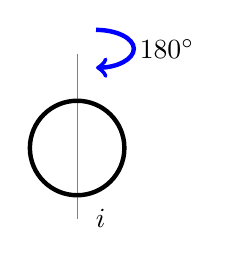
\begin{tikzpicture}[scale=0.6]
\draw[gray] (0,-1.5)--(0,2);

 \draw[ultra thick]  (0:1) arc (0:360:1);
\draw[->,ultra thick,blue]  (0.4,2.5) arc (90:-90:0.8 and 0.4) ;

 \node at (0.5,-1.5) {$i$}; 
 \node at (1.9,2.1) {$180^ \circ$};
\end{tikzpicture}

 \caption{The move $\rho_i$ (left).
 The move $\sigma_i$ (center).
 The move $\tau_i$ (right).
 \label{fig:moves}}
\end{figure}

The move $\rho_i$ is the path permuting the $i$-th and the $i+1$-th circles by passing over (or around)
while $\sigma_i$ permutes them by passing the $i$-th circle through the $i+1$-th and $\tau_i$ is a $180^\circ$ rotation of the circle back to itself, 
which verifies $\tau_i^2 = {\mathop{\mathrm{id}}\nolimits}$ (see \cite{BH}, with reverse notation for $\sigma_i$ and $\rho_i$, see also \cite{FS}). 
To avoid the last move $\tau_i$   one can define
$\mathcal{UR}_n$ as the configuration of $n$ unlinked Euclidean circles being all parallel to a fixed plane, say the $yz$-plane
(\emph{untwisted rings}).
The fundamental group of this configuration space is denoted in \cite{BH} by $UR_n$ but we will denote it by $WB_n$
and we shall call it  {\emph{{welded braid group}}}, since this is the most usual name for  this group  which appears in the literature in other  different contexts such as
motion groups (\cite{G1},\cite{G2}), ribbon tubes (\cite{ABMW})
automorphisms of free groups (\cite{BP,FRR}) 
or collections of paths (\cite{FRR}).

\bigskip

This article is devoted to the relationship between   configuration spaces of points 
over an annulus and configuration spaces of Euclidean circles.
We will introduce the configuration space of a special link, composed with Euclidean circles, called the 
{\emph{{necklace}}} and denoted by $\mathcal{L}_n$ and we will consider  induced representations as automorphisms of free groups.
\begin{figure}
 
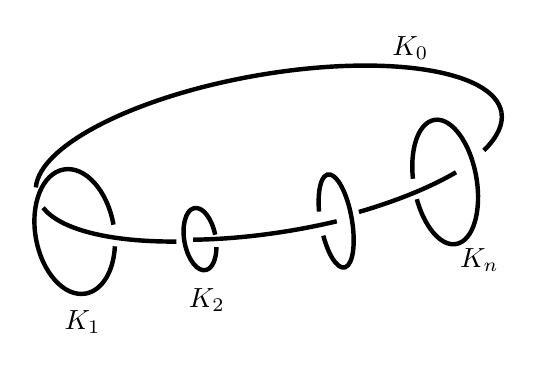
\begin{tikzpicture}[scale=1]

\begin{scope}[rotate=10]

\draw[ultra thick] (3,0) arc (0:175:3 and 1);
\draw[ultra thick] (3,0) arc (0:-26:3 and 1);
\draw[ultra thick] (2.3,-0.65) arc (-42:-72:3 and 1) ;
\draw[ultra thick] (0.7,-1) arc (-80:-116:3 and 1) ;
\draw[ultra thick]  (-1.35,-0.9) arc (-117:-170:3 and 1) ;

 \node at (2,1) {$K_0$}; 

 \node at (-2.7,-1.7) {$K_1$}; 
\draw[ultra thick] (-2.1,-0.55) arc (0:340:0.5 and 0.8);

 \node at (-1.1,-1.7) {$K_2$}; 
\draw[ultra thick] (-0.85,-0.90) arc (3:340:0.2 and 0.4);

\draw[ultra thick] (0.5,-1.15) arc (-165:165:0.2 and 0.6);

 \node at (2.4,-1.8) {$K_n$}; 
\draw[ultra thick] (1.75,-0.9) arc (-169:172:0.4 and 0.8);

\end{scope}

\end{tikzpicture}
 
 \caption{The necklace $\mathcal{L}_n$.\label{fig:necklace}}
\end{figure}

Our first result (Theorem \ref{th:circular}) is that the fundamental group of the configuration space of $n$ components necklaces (that we will call  \emph{braid group of a necklace})
is isomorphic to 
the fundamental group of the configuration space of $n$ points 
over an annulus (which is $CB_n$)  quotiented by the square of its center.  

A theorem of Artin characterizes automorphisms of a free group coming 
from the action of the standard braid group. In our case, to a loop $\mathcal{L}_n(t)$ of necklaces we associate
an automorphism from $\pi_1({\mathbb{R}}^3\setminus\mathcal{L}_n)$ to itself.
Our second result, Theorem \ref{th:circularartin},  is an analogous of Artin's theorem for the braid group of a necklace.

In section \ref{sec:zero}, we define affine braid groups of type $\mathcal{A}$ in terms of configurations of Euclidean circles
and we refine the representation given  in Theorem \ref{th:circularartin} to obtain
 a faithful representation and a characterization as automorphisms of free groups for affine braid groups of type $\mathcal{A}$ (Theorem \ref{thm:affine}):
 this is the third main result of the paper.
In section \ref{ssec:linearnecklace} we show how to define the braid group $B_n$
 in terms of configurations of Euclidean circles and we give a short survey on some remarkable (pure) subgroups
 of $WB_n$; finally,  in the Appendix we find the kernel of a particular representation of $CB_n$ in ${\mathop{\mathrm{Aut}}\nolimits} F_n$, proving this way the statement of Theorem
 \ref{thmCB}, which plays a key role in the proof of  Theorem \ref{thm:affine}.

\section{Necklaces and circular braids}
\label{sec:necklace}

\subsection{The circular braid group}

Recall that the circular braid group $CB_n$ is the fundamental group
of $n$ distinct points in the plane less the origin (i.e.~topologically an annulus).
The circular braid group $CB_n$
admits the following  presentation (where the indices are defined modulo $n$, see for instance \cite{KP}):
$$CB_n = \left\langle \sigma_1,\ldots,\sigma_n, \zeta \mid
\begin{array}{l}
\sigma_i\sigma_{i+1}\sigma_i = \sigma_{i+1}\sigma_i\sigma_{i+1} \quad \text{ for } i = 1,2\ldots, n, \\
\sigma_i\sigma_j=\sigma_j\sigma_i \quad \text{ for } |i-j| \neq 1, \\
{\bar{{\zeta}}} \sigma_i \zeta =\sigma_{i+1} \quad \text{ for } i = 1,2\ldots, n \\
\end{array}
\right\rangle.
$$
where ${\bar{{\zeta}}}$ stands for $\zeta^{-1}$.
Geometrically $\sigma_i$ consists in permuting the $i$-th and $i+1$-th point and $\zeta$ in a cyclic permutation
of the points.

\begin{figure}
 
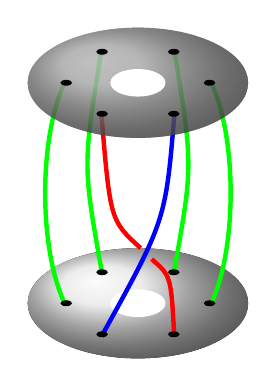
\begin{tikzpicture}[scale=0.7]
\fill [ball color=gray!20] (0,0) ellipse (2 and 1);
\fill [white] (0,0) ellipse (0.5 and 0.25);

\draw[ultra thick,blue]  (-0.66,-0.6)  .. controls (0.5,1.5).. (0.66,3.4);

\draw[ultra thick,red] (0.66,-0.6) .. controls (0.6,0.5)  .. (0.25,0.8);
\draw[ultra thick,red] (0.05,1) .. controls (-0.5,1.5)  .. (-0.66,3.4);

\draw[ultra thick,green] (-1.33,0).. controls (-1.8,1)  and (-1.8,3)   ..(-1.33,4);

\draw[ultra thick,green] (1.33,0).. controls (1.8,1)  and (1.8,3)   ..(1.33,4);

\draw[ultra thick,green] (0.66,0.6) .. controls (1,2.5)  .. (0.66,4.6);

\draw[ultra thick,green] (-0.66,0.6)  .. controls (-1,2.5)  .. (-0.66,4.6);

\fill [ball color=gray!20,opacity=0.6] (0,4) ellipse (2 and 1);
\fill [white] (0,4) ellipse (0.5 and 0.25);

\begin{scope}[yscale=0.5]
\foreach \i in{0,60,...,300}{
  \fill[black,opacity=1]({\i}:1.3) circle(3pt);
  \fill[black,opacity=1] (0,8)+({\i}:1.3) circle(3pt);
};
\end{scope}

\end{tikzpicture}
 \qquad\qquad
 
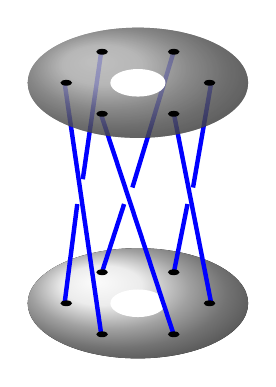
\begin{tikzpicture}[scale=0.7]
\fill [ball color=gray!20] (0,0) ellipse (2 and 1);
\fill [white] (0,0) ellipse (0.5 and 0.25);

\draw[ultra thick,blue]  (0.66,-0.6)  -- (-0.66,3.4);

\draw[ultra thick,blue]  (-0.66,-0.6)  -- (-1.33,4);

\draw[ultra thick,blue]  (1.33,0)  -- (0.66,3.4);

\draw[ultra thick,blue]  (0.66,0.6)  -- (0.9,1.8);
\draw[ultra thick,blue]  (1,2.1)  -- (1.33,4);

\draw[ultra thick,blue]  (-0.64,0.6)  -- (-0.25,1.8);
\draw[ultra thick,blue]  (-0.1,2.1)  -- (0.66,4.6);

\draw[ultra thick,blue]  (-1.33,0)  -- (-1.1,1.8);
\draw[ultra thick,blue]  (-1,2.25)  -- (-0.66,4.6);

\fill [ball color=gray!20,opacity=0.6] (0,4) ellipse (2 and 1);
\fill [white] (0,4) ellipse (0.5 and 0.25);

\begin{scope}[yscale=0.5]
\foreach \i in{0,60,...,300}{
  \fill[black,opacity=1]({\i}:1.3) circle(3pt);
  \fill[black,opacity=1] (0,8)+({\i}:1.3) circle(3pt);
};
\end{scope}

\end{tikzpicture}

 \caption{A move $\sigma_i$ (left). 
 The move $\zeta$ (right).}
\end{figure}

This is closed to a presentation of the classical braid group, with two major differences:
(a) the indices are defined modulo $n$; (b) there are additional relations ${\bar{{\zeta}}} \sigma_i \zeta =\sigma_{i+1}$.
In fact these latter relations enable to generate $CB_n$
with only two generators: $\sigma_1$ and $\zeta$.
We will consider the (well defined) representation $\rho_{CB}:  CB_n \to {\mathop{\mathrm{Aut}}\nolimits} F_n$   defined as follows: 
$$\rho_{CB}(\sigma_i) : 
\left\{\begin{array}{l}
x_i \mapsto x_{i} x_{i+1} {\bar{{x_{i}}}} \\
x_{i+1} \mapsto x_i \\
x_{j} \mapsto x_j \quad j \neq i,i+1\\
\end{array}\right.
\qquad 
\rho_{CB}(\zeta) : 
\left\{\begin{array}{l}
x_j \mapsto x_{j+1} \\      
\end{array}\right.$$
where indices are modulo $n$.
The following Theorem will be proved in the Appendix and will play a key role in next sections.

\begin{theorem} \label{thmCB}
The kernel of $\rho_{CB}:  CB_n \to {\mathop{\mathrm{Aut}}\nolimits} F_n$ is the cyclic group generated by $\zeta^n$.
\end{theorem}

\subsection{Necklaces} Let $\mathcal{L}_n = K_0 \cup K_1 \cup  \ldots\cup K_n$ be the following link : 

\begin{figure}
 
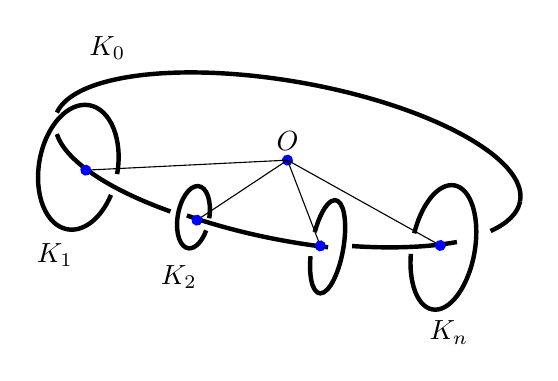
\begin{tikzpicture}[scale=1]

\begin{scope}[rotate=-10]

\draw[ultra thick] (3,0) arc (0:175:3 and 1);
\draw[ultra thick] (3,0) arc (0:-26:3 and 1);
\draw[ultra thick] (2.3,-0.65) arc (-42:-72:3 and 1) ;
\draw[ultra thick] (0.7,-1) arc (-80:-116:3 and 1) ;
\draw[ultra thick]  (-1.35,-0.9) arc (-117:-170:3 and 1) ;

 \node at (-2.5,1) {$K_0$}; 
 \fill[blue] (0,0) circle (2pt);
 \node[above] at (0,0) {$O$};

 \node at (-2.7,-1.7) {$K_1$}; 
\draw (0,0) --(-2.5,-0.57);
\fill[blue](-2.5,-0.57) circle (2pt);
\draw[ultra thick] (-2.1,-0.55) arc (0:340:0.5 and 0.8);

 \node at (-1.1,-1.7) {$K_2$}; 
\draw (0,0) -- (-1,-0.95);
\fill[blue] (-1,-0.95) circle (2pt);
\draw[ultra thick] (-0.85,-0.90) arc (3:340:0.2 and 0.4);

\draw (0,0) -- (0.6,-1.0) ;
\fill[blue] (0.6,-1) circle (2pt);
\draw[ultra thick] (0.5,-1.15) arc (-165:165:0.2 and 0.6);

 \node at (2.4,-1.8) {$K_n$}; 
\draw (0,0) -- (2.1,-0.73);
 \fill[blue] (2.1,-0.73) circle (2pt);
\draw[ultra thick] (1.75,-0.9) arc (-169:172:0.4 and 0.8);

\end{scope}

\end{tikzpicture}
 
 \caption{The necklace $\mathcal{L}_n$.
 \label{fig:necklacebis}}
\end{figure}

A link is called a {\emph{{necklace}}} if:
\begin{itemize}
  \item $K_0$ is an Euclidean circle of center $O$ and of radius $1$,
  
  \item each Euclidean circle $K_i$ has a center $O_i$ belonging to $K_0$,
  the circle $K_i$ being of radius $r_i$ with $0 < r_i < \frac12$
  and belonging to the plane containing the line $(OO_i)$ and perpendicular to 
  the plane of $K_0$,
  
  \item if $O_i=O_j$ then $r_i \neq r_j$.
\end{itemize}
We will suppose $n{\geqslant}2$ and that the link is oriented.

\bigskip

In particular each $K_i$ is a trivial knot such that:
\begin{equation*}
\left\{\begin{array}{ll}
{\mathop{\mathrm{lk}}\nolimits}(K_0,K_i)=+1  &\quad i=1,\ldots,n \\
{\mathop{\mathrm{lk}}\nolimits}(K_i,K_j)=0   &\quad i,j = 1,\ldots,n, \ \ i\neq j \\
\end{array}\right.
\end{equation*}

\subsection{The iteration $\tau^n$}

 

Let $\tau \in \pi_1({\mathop{\mathrm{Conf}}\nolimits} \mathcal{L}_n)$ denote the circular permutation of 
circles $K_1 \to K_2$, $K_2 \to K_3$,\ldots
It is important to understand the iteration $\tau^n$. 
We give two visions of $\tau^n$ in $\pi_1({\mathop{\mathrm{Conf}}\nolimits} \mathcal{L}_n)$.
\begin{itemize}
  \item This move can of course be seen as $n$ iterations of $\tau$: so that it is a 
full rotation of all the $K_i$ ($i=1,\ldots,n$) along $K_0$, back to their initial position.
  \item $\tau^n$ can be seen in another way: suppose that $K_1,\ldots,K_n$ are 
  sufficiently closed circles. Fixing those $K_i$, $\tau^n$ corresponds to a full rotation of $K_0$
around all the $K_i$. 
\end{itemize}
Indeed each of this move is rotation of angle $2\pi$ around an axis, 
and we can continuously change the axis to go from the first vision to the second.

\begin{figure}
 
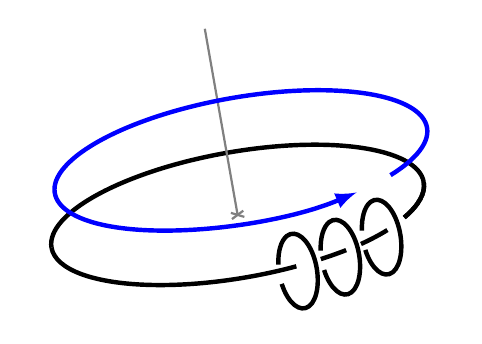
\begin{tikzpicture}[scale=0.8]

\begin{scope}[rotate=10]
\draw[ultra thick] (3,0) arc (0:180:3 and 1);

\draw[gray,thick] (0,0)--+(0.1,0.05)--+(-0.1,-0.05);
\draw[gray,thick] (0,0)--+(-0.1,0.05)--+(0.1,-0.05);
\draw[gray,thick] (0,-0)--(0,3);

\draw[ultra thick] (3,0) arc (0:-30:3 and 1);
\draw[ultra thick] (3,0) arc (0:-30:3 and 1); 
\draw[ultra thick] (2.3,-0.65) arc (-40:-52:3 and 1) ;
\draw[ultra thick] (1.6,-0.85) arc (-59:-68:3 and 1) ;
\draw[ultra thick] (-3,0) arc (-180:-75:3 and 1) ;

\draw[ultra thick] (0.5,-1.2) arc (-165:165:0.3 and 0.6);
\draw[ultra thick] (1.2,-1.1) arc (-165:165:0.3 and 0.6);
\draw[ultra thick] (1.9,-0.9) arc (-165:165:0.3 and 0.6);

\draw[->,>=latex,ultra thick,blue] (2.5,0.2)  arc (-40:305:3 and 1);

\end{scope}

\end{tikzpicture}
\qquad
 
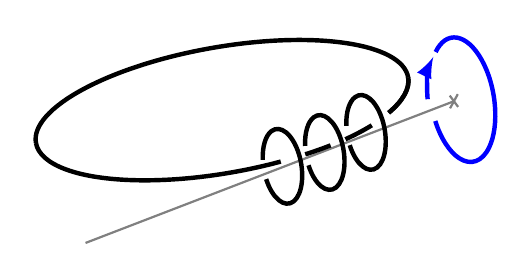
\begin{tikzpicture}[scale=0.8]

\begin{scope}[rotate=10]
\draw[ultra thick] (3,0) arc (0:180:3 and 1);
\draw[gray,thick] (-2.5,-1.7)--(3.65,-0.5);

\draw[gray,thick] (3.65,-0.5)--+(0.08,0.1)--+(-0.08,-0.1);
\draw[gray,thick] (3.65,-0.5)--+(0.05,-0.1)--+(-0.05,0.1);

\draw[ultra thick] (3,0) arc (0:-30:3 and 1);
\draw[ultra thick] (3,0) arc (0:-30:3 and 1); 
\draw[ultra thick] (2.3,-0.65) arc (-40:-52:3 and 1) ;
\draw[ultra thick] (1.6,-0.85) arc (-59:-68:3 and 1) ;
\draw[ultra thick] (-3,0) arc (-180:-75:3 and 1) ;

\draw[ultra thick] (0.5,-1.2) arc (-165:165:0.3 and 0.6);
\draw[ultra thick] (1.2,-1.1) arc (-165:165:0.3 and 0.6);
\draw[ultra thick] (1.9,-0.9) arc (-165:165:0.3 and 0.6);

\draw[ultra thick,blue] (3.5,0.32)  arc (125:-165:0.5 and 1);
\draw[<-,>=latex,ultra thick,blue] (3.45,0.25)  arc (125:170:0.5 and 1);

\end{scope}

\end{tikzpicture}

 \caption{Two visions of $\tau^n$. \label{fig:taun}}
\end{figure}

\subsection{The fundamental group of ${\mathop{\mathrm{Conf}}\nolimits} \mathcal{L}_n$}
\label{ssec:pi1}

\begin{theorem}
\label{th:circular}
For $n{\geqslant} 2$, the group  $\pi_1({\mathop{\mathrm{Conf}}\nolimits} \mathcal{L}_n)$ is isomorphic 
to the circular braid group $CB_n/\langle \zeta^{2n} \rangle$.  
\end{theorem}

\begin{proof}
We start with a rigid configuration  where
$K_0^*$ is the Euclidean circle in the plane $(Oxy)$ centered at $O$
and of radius $1$. A necklace having such a core circle $K_0^*$
is called a {\emph{{normalized necklace}}} and we denote it by $\mathcal{L}_n^*$. 
  
\begin{lemma}
\label{lem:cbn}
${\mathop{\mathrm{Conf}}\nolimits} \mathcal{L}_n^*$ is homeomorphic to the configuration space $\mathcal{CB}_n$.  
\end{lemma}

\begin{proof}[Proof of the lemma]
We consider  $\mathcal{CB}_n$ as the configuration space of $n$
points lying on the annulus $A_0 = D_1 \setminus D_{\frac12}$, 
where $D_r$ denotes the closed disk in the plane $(Oxy)$ centered at $O$ of radius $r$.
To a normalized necklace $\mathcal{L}_n^*$ we associate $n$ points of $A_0$ as follows:
$$(K_1,\ldots,K_n) \longmapsto (K_1 \cap A_0, \ldots,K_n \cap A_0 ).$$
As each point of $A_0$ determines a unique normalized circle $K_i$,
this map is a bijection. This maps and its inverse are continuous.
\end{proof}  
  

We end the proof of Theorem \ref{th:circular} as follows.
To a necklace $\mathcal{L}_n$ having core circle $K_0$
we associate a unit vector $u_0$, orthogonal to the plane containing
$K_0$ (and oriented according to the orientation of $K_0$).

\begin{figure}
 
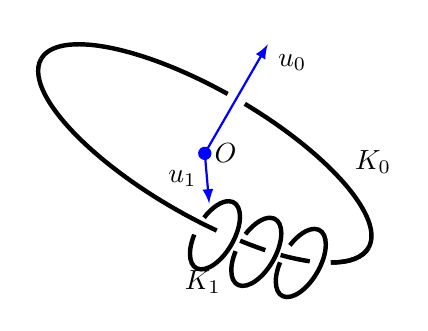
\begin{tikzpicture}[scale=0.8]

\begin{scope}[rotate=-30]

\draw[ultra thick] (3,0) arc (0:87:3 and 1);
\draw[ultra thick] (-3,0) arc (0:87:-3 and 1);

\draw[->,>=latex,blue, thick] (0,-0)--(0,2) node[black, below right] {$u_0$};
\draw[->,>=latex,blue, thick] (0,-0)--(-55:0.8) node[midway, black,left] {$u_1$};
\fill[blue] (0,0) circle (3pt) node[black, right]{$O$};
\node[right] at (2,1) {$K_0$}; 
\node[right] at (-73:2.1) {$K_1$}; 

\draw[ultra thick] (3,0) arc (0:-30:3 and 1);
\draw[ultra thick] (3,0) arc (0:-30:3 and 1); 
\draw[ultra thick] (2.3,-0.65) arc (-40:-52:3 and 1) ;
\draw[ultra thick] (1.6,-0.85) arc (-59:-68:3 and 1) ;
\draw[ultra thick] (-3,0) arc (-180:-75:3 and 1) ;

\draw[ultra thick] (0.5,-1.2) arc (-165:165:0.3 and 0.6);
\draw[ultra thick] (1.2,-1.1) arc (-165:165:0.3 and 0.6);
\draw[ultra thick] (1.9,-0.9) arc (-165:165:0.3 and 0.6);

\end{scope}

\end{tikzpicture}
 
 \caption{The normal vector $u_0$. \label{fig:uzero}}
\end{figure}

Let $G : {\mathop{\mathrm{Conf}}\nolimits}(\mathcal{L}_n) \to S^2$ be the map defined
by $G(\mathcal{L}_n) = u_0$. This map $G$ is a locally trivial fibration
whose fiber is ${\mathop{\mathrm{Conf}}\nolimits} \mathcal{L}_n^*$ (for the unit vector $u_0 = (0,0,1)$).
The long exact sequence in homotopy for the fibration 
${\mathop{\mathrm{Conf}}\nolimits} \mathcal{L}_n^* \hookrightarrow {\mathop{\mathrm{Conf}}\nolimits} \mathcal{L}_n \twoheadrightarrow S^2$
provides:
$$
\begin{array}{c}
0 
\longrightarrow \pi_2({\mathop{\mathrm{Conf}}\nolimits} \mathcal{L}_n^*)
\overset{H_2}{\longrightarrow} \pi_2({\mathop{\mathrm{Conf}}\nolimits} \mathcal{L}_n)
\overset{G_2}{\longrightarrow} \pi_2(S^2) \\
\qquad\qquad \overset{d}{\longrightarrow} \pi_1({\mathop{\mathrm{Conf}}\nolimits} \mathcal{L}_n^*)
\overset{H_1}{\longrightarrow} \pi_1({\mathop{\mathrm{Conf}}\nolimits} \mathcal{L}_n)
\longrightarrow 0
\end{array}$$
It implies that $H_1$ is surjective (since in the exact sequence $\pi_1(S^2)$ is trivial).

\bigskip

Before computing the kernel of $H_1$, we give a motivation why $H_1$ is not injective.
There is a natural map $K$ from ${\mathop{\mathrm{Conf}}\nolimits} \mathcal{L}_n$ to $SO_3$.
Let us see $SO_3$ as the space of direct orthonormal frames $(u_0,u_1,u_2)$.
To a necklace $\mathcal{L}_n$ we associate $u_0$ as above, while $u_1$ is the unit vector
from the origin $O$ to $K_1$, then we set $u_2 = u_0 \wedge u_1$ (see figure \ref{fig:uzero}). 

Let us denote by $\pi : SO_3 \to S^2$,  the natural projection 
$\pi(u_0,u_1,u_2) = u_0$. 
We have a commutative diagram, that is to say $G = \pi \circ K$.
But as $\pi_2(SO_3) = 0$, it implies $G_2 = 0$. By the exact sequence, $d$ is injective, so that
$\pi_2(S^2) = {\mathbb{Z}} \cong {\mathop{\mathrm{Im}}\nolimits} d = {\mathop{\mathrm{Ker}}\nolimits} H_1$.

There is another interesting point with $SO_3$. In fact if we now see $SO_3$ 
as the space of rotations, we denote 
by $\rho$ a full rotation around the vertical axis (supported by $u_0$).
The $\rho \neq {\mathop{\mathrm{id}}\nolimits}$, but $\rho^2 \simeq {\mathop{\mathrm{id}}\nolimits}$ (because $\pi_1(SO_3) \cong {\mathbb{Z}}/2{\mathbb{Z}}$).
For us the move $\rho$ corresponds to the full rotation $\tau^n$. 
It gives the idea that in ${\mathop{\mathrm{Conf}}\nolimits} \mathcal{L}_n^*$, $\tau^n$ generates a subgroup isomorphic to 
 ${\mathbb{Z}}$, but $\tau^{2n}$ is homotopic to ${\mathop{\mathrm{id}}\nolimits}$ in ${\mathop{\mathrm{Conf}}\nolimits} \mathcal{L}_n$.

\bigskip
 
We will now compute the kernel of $H_1$ as ${\mathop{\mathrm{Im}}\nolimits} d$, where $d$ is the boundary map 
coming from the exact sequence : ${\mathop{\mathrm{Ker}}\nolimits} H_1 = \langle \tau^{2n} \rangle$.

We go back to the construction of this boundary map $d$ (see for instance,
\cite[Theorem 6.12]{Hu}) and we explicit one of the lifting.
Let $f$ be the generator of $\pi_2(S^2) \cong {\mathbb{Z}}$ defined by 
$f : S^2 \to S^2$, $f(x)=x$, but we prefer to see it as a map 
$$f : I \times I \to S^2 \quad \text{such that}\quad f(\partial I^2) = N$$
where $N=(0,0,1)$ is the North pole of $S^2$.

We lift $f$ to a map $\tilde f$ from $\partial I \times I \cup I \times \{0\}$
to the base-point $\mathcal{L}_n^*$ in ${\mathop{\mathrm{Conf}}\nolimits} \mathcal{L}_n$ (and ${\mathop{\mathrm{Conf}}\nolimits} \mathcal{L}_n^*$, for which 
$u_0$ is $\overrightarrow{ON}$).

By the homotopy lifting property, it extends to a map
$h : I\times I \to {\mathop{\mathrm{Conf}}\nolimits} \mathcal{L}_n$,
and $d(f) \in \pi_1({\mathop{\mathrm{Conf}}\nolimits} \mathcal{L}_n^*)$ is the map 
induced by $h_{|I\times \{1\}}$ (figure \ref{fig:lift}).

\begin{figure}
 
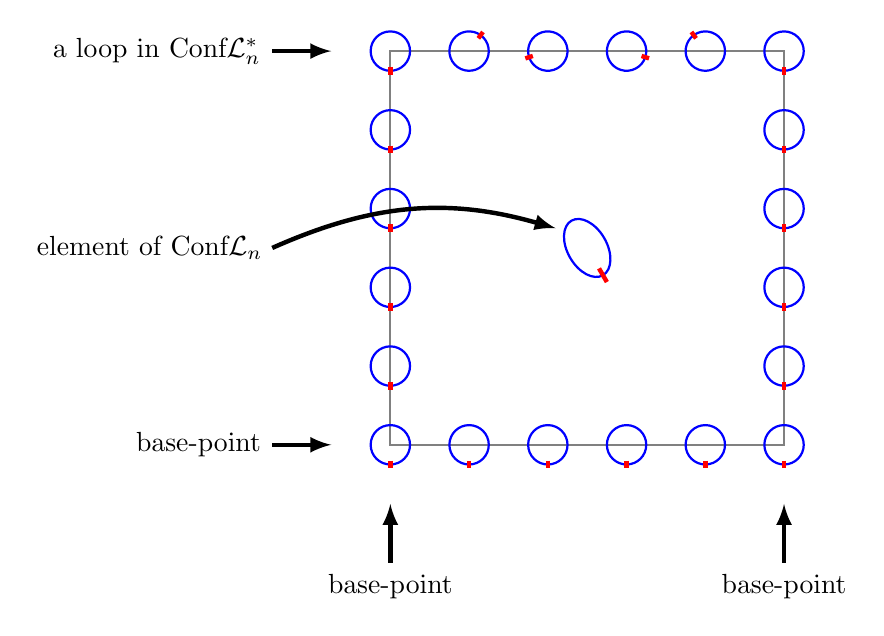
\begin{tikzpicture}[scale=0.5]

\draw[thick, gray] (0,0) rectangle (10,10);

  \foreach \r in {0,2,...,10} {
      \begin{scope}[xshift=\r cm]
           {
  \draw[blue, thick] (0,0) circle(0.5); 
  \draw[ultra thick, red] (0,-0.4)--(0,-0.6);
}
       \end{scope}
    }
  \foreach \r in {2,4,...,10} {
      \begin{scope}[yshift=\r cm]
           {
  \draw[blue, thick] (0,0) circle(0.5); 
  \draw[ultra thick, red] (0,-0.4)--(0,-0.6);
}
       \end{scope}
    }
  \foreach \r in {2,4,...,10} {
      \begin{scope}[xshift=10cm,yshift=\r cm]
           {
  \draw[blue, thick] (0,0) circle(0.5); 
  \draw[ultra thick, red] (0,-0.4)--(0,-0.6);
}
       \end{scope}
    }
  \foreach \r in {2,4,6,8} {
      \begin{scope}[xshift=\r cm, yshift = 10cm, rotate=72*\r]
           {
  \draw[blue, thick] (0,0) circle(0.5); 
  \draw[ultra thick, red] (0,-0.4)--(0,-0.6);
}
       \end{scope}
    }

\begin{scope}[xshift=5 cm,yshift=5 cm, rotate=30]
  \draw[blue,thick] (0,0) ellipse(0.5 and 0.8); 
  \draw[ultra thick, red] (0,-0.6)--(0,-1);
\end{scope}

\draw[->,>=latex,ultra thick] (0,-3)--+(0,1.5) node[pos=0, below] {base-point};
\draw[->,>=latex,ultra thick] (10,-3)--+(0,1.5) node[pos=0, below] {base-point};
\draw[->,>=latex,ultra thick] (-3,0)--+(1.5,0) node[pos=0, left] {base-point};
\draw[->,>=latex,ultra thick] (-3,10)--+(1.5,0) node[pos=0, left] {a loop in $\text{Conf}\mathcal{L}_n^*$};
\draw[->,>=latex,ultra thick] (-3,5) to[bend left = 20] (4.2,5.5);
\node[left] at (-3,5) {element of $\text{Conf} \mathcal{L}_n$};

\end{tikzpicture}

 \caption{\label{fig:lift}The lifting $h$ from $I\times I$ to ${\mathop{\mathrm{Conf}}\nolimits} \mathcal{L}_n$ ($K_0$ in blue, $K_1$ in red).}
\end{figure}

One way to explicit this lifting is to see $I^2 \setminus \partial I^2$ as $S^2 \setminus \{N\}$.
On $S^2$ there exists a continuous vector field, 
that is non-zero except at $N$ (see the dipole integral curves in figure \ref{fig:dipole}, see also \cite[section 5]{CaPa} 
for other links between vector fields and configuration spaces).
Now at each point $u_0 \in S^2 \setminus \{N\}$ is associated a non-zero vector $u_1$.
Let us define $h : S^2 \setminus \{N\} \to {\mathop{\mathrm{Conf}}\nolimits} \mathcal{L}_n$
as follows: for $u_0 \in S^2\setminus \{N\}$, $h(u_0)$ is the unique
necklace $\mathcal{L}_n$, such $G(\mathcal{L}_n) = u_0$ and
the unit vector from $O$ to $K_1$ is $u_1$. We define $K_2,\ldots,K_n$ as parallel copies of $K_1$
(figure \ref{fig:neck}).
\begin{figure}
 
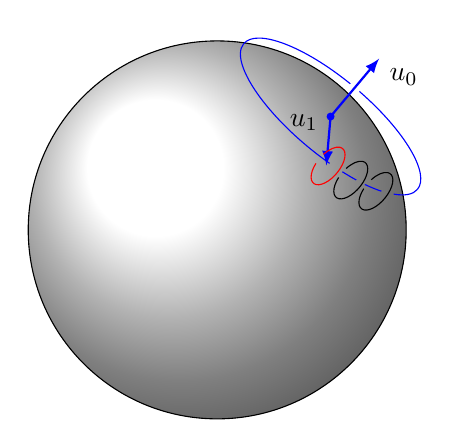
\begin{tikzpicture}[scale=1.2]

\filldraw[ball color=white] (0,0) circle (2);

\begin{scope}[scale = 0.4, xshift=3cm,yshift=3cm, rotate=-40,]

\draw[blue] (3,0) arc (0:87:3 and 1);
\draw[blue] (-3,0) arc (0:87:-3 and 1);

\draw[->,>=latex,blue, thick] (0,-0)--(0,2) node[black, below right] {$u_0$};
\draw[->,>=latex,blue, thick] (0,-0)--(-55:1.3) node[midway, black,above left] {$u_1$};
\fill[blue] (0,0) circle (3pt); 

\draw[blue] (3,0) arc (0:-30:3 and 1); 
\draw[blue] (2.3,-0.65) arc (-40:-52:3 and 1) ;
\draw[blue] (1.6,-0.85) arc (-59:-68:3 and 1) ;
\draw[blue] (-3,0) arc (-180:-75:3 and 1) ;

\draw[red] (0.5,-1.2) arc (-165:165:0.3 and 0.6);
\draw (1.2,-1.1) arc (-165:165:0.3 and 0.6);
\draw (1.9,-0.9) arc (-165:165:0.3 and 0.6);

\end{scope}

\end{tikzpicture}

 \caption{\label{fig:neck}A necklace constructed from $u_0 \in S^2$ and $u_1 \in T_{u_0} S^2$.}
\end{figure}

Now $d(f)$ corresponds to the lift $h(\gamma)$ where $\gamma$ is a small loop in $S^2$ around $N$.
Due to the dipole figure at $N$, $h(\gamma)$ is exactly $\tau^{2n}$ (figures \ref{fig:vector} and \ref{fig:tau2n}).

\begin{figure}
 
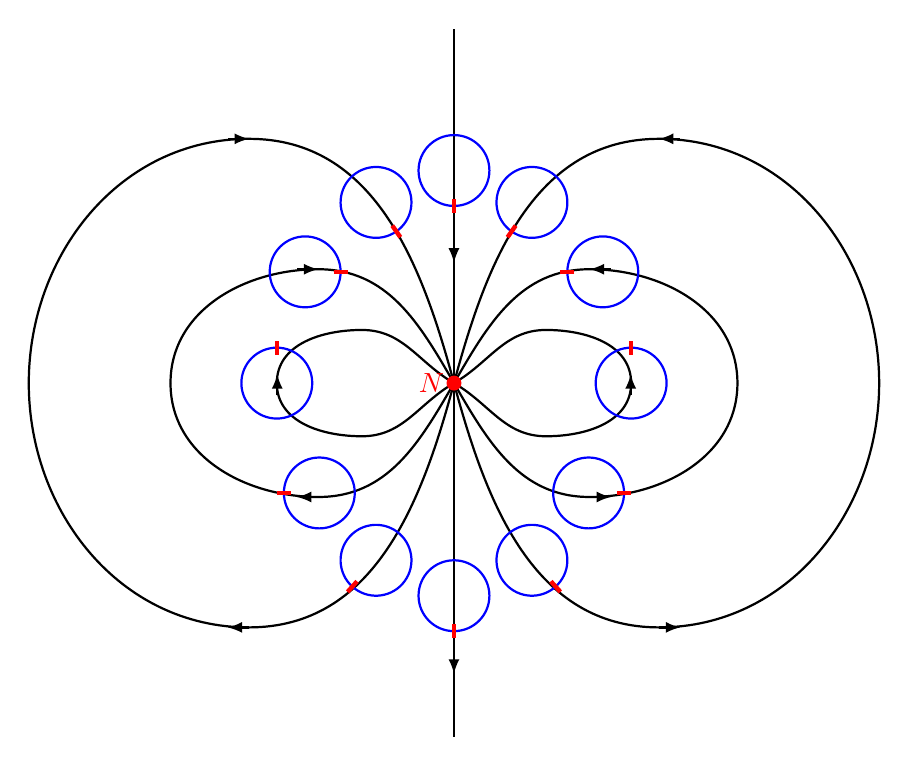
\begin{tikzpicture}[scale=0.9]

\draw[thick] (0,0) to [out=-60,in=180] (-40:2.5) to [out=0,in=-90] (0:4);
\draw[thick] (0,0) to [out=-75,in=180] (-50:4.5) to [out=0,in=-90] (0:6);
\draw[thick] (0,0) to (-90:5);
\draw[thick] (0,0) to [out=-30,in=180] (-30:1.5) to [out=0,in=-90] (0:2.5);

\begin{scope}[cm={1,0,0,-1,(0,0)}]
  \draw[thick]  (0,0) to [out=-60,in=180] (-40:2.5) to [out=0,in=-90] (0:4);
  \draw[thick] (0,0) to [out=-75,in=180] (-50:4.5) to [out=0,in=-90] (0:6);
  \draw[thick] (0,0) to (-90:5);
  \draw[thick] (0,0) to [out=-30,in=180] (-30:1.5) to [out=0,in=-90] (0:2.5);
\end{scope}

\begin{scope}[cm={-1,0,0,-1,(0,0)}]
  \draw[thick]  (0,0) to [out=-60,in=180] (-40:2.5) to [out=0,in=-90] (0:4);
  \draw[thick] (0,0) to [out=-75,in=180] (-50:4.5) to [out=0,in=-90] (0:6);
  \draw[thick] (0,0) to (-90:5);
  \draw[thick] (0,0) to [out=-30,in=180] (-30:1.5) to [out=0,in=-90] (0:2.5);
\end{scope}

\begin{scope}[cm={-1,0,0,1,(0,0)}]
  \draw[thick]  (0,0) to [out=-60,in=180] (-40:2.5) to [out=0,in=-90] (0:4);
  \draw[thick] (0,0) to [out=-75,in=180] (-50:4.5) to [out=0,in=-90] (0:6);
  \draw[thick] (0,0) to (-90:5);
  \draw[thick] (0,0) to [out=-30,in=180] (-30:1.5) to [out=0,in=-90] (0:2.5);
\end{scope}

\draw[->,>=latex,thick] (-90:3.8)--+(0,-0.3);
\draw[->,>=latex,thick] (90:2)--+(0,-0.3);
\draw[->,>=latex,thick] (-4:2.5)--+(0,0.3);
\draw[->,>=latex,thick] (4:-2.5)--+(0,0.3);

\draw[->,>=latex,thick] (-40:2.5)--+(0.3,0);
\draw[<-,>=latex,thick] (40:2.5)--+(0.3,0);

\draw[->,>=latex,thick] (-50:4.5)--+(0.3,0);
\draw[<-,>=latex,thick] (50:4.5)--+(0.3,0);

\begin{scope}[cm={-1,0,0,1,(0,0)}]
\draw[->,>=latex,thick] (-40:2.5)--+(0.3,0);
\draw[<-,>=latex,thick] (40:2.5)--+(0.3,0);

\draw[->,>=latex,thick] (-50:4.5)--+(0.3,0);
\draw[<-,>=latex,thick] (50:4.5)--+(0.3,0);
\end{scope}

\fill[red] (0,0) circle (3pt) node[left]{$N$};

 \begin{scope}[yshift=-3 cm] {
  \draw[blue, thick] (0,0) circle(0.5); 
  \draw[ultra thick, red] (0,-0.4)--(0,-0.6);
}  \end{scope}
 \begin{scope}[yshift=3 cm] {
  \draw[blue, thick] (0,0) circle(0.5); 
  \draw[ultra thick, red] (0,-0.4)--(0,-0.6);
}  \end{scope}

 \begin{scope}[xshift = 1.1cm, yshift=-2.5 cm,rotate = 42] {
  \draw[blue, thick] (0,0) circle(0.5); 
  \draw[ultra thick, red] (0,-0.4)--(0,-0.6);
}  \end{scope}
 \begin{scope}[xshift = 1.9cm, yshift=-1.55 cm,rotate = 90] {
  \draw[blue, thick] (0,0) circle(0.5); 
  \draw[ultra thick, red] (0,-0.4)--(0,-0.6);
}  \end{scope}
 \begin{scope}[xshift = 2.1cm, yshift=1.57 cm,rotate = -90] {
  \draw[blue, thick] (0,0) circle(0.5); 
  \draw[ultra thick, red] (0,-0.4)--(0,-0.6);
}  \end{scope}
 \begin{scope}[xshift = 1.1cm, yshift=2.55 cm,rotate = -35] {
  \draw[blue, thick] (0,0) circle(0.5); 
  \draw[ultra thick, red] (0,-0.4)--(0,-0.6);
}  \end{scope}

 \begin{scope}[xshift = 2.5cm, yshift=0 cm,rotate = 180] {
  \draw[blue, thick] (0,0) circle(0.5); 
  \draw[ultra thick, red] (0,-0.4)--(0,-0.6);
}  \end{scope}

 \begin{scope}[xshift = -1.1cm, yshift=-2.5 cm,rotate = -42] {
  \draw[blue, thick] (0,0) circle(0.5); 
  \draw[ultra thick, red] (0,-0.4)--(0,-0.6);
}  \end{scope}
 \begin{scope}[xshift = -1.9cm, yshift=-1.55 cm,rotate = -90] {
  \draw[blue, thick] (0,0) circle(0.5); 
  \draw[ultra thick, red] (0,-0.4)--(0,-0.6);
}  \end{scope}
 \begin{scope}[xshift = -2.1cm, yshift=1.57 cm,rotate = 90] {
  \draw[blue, thick] (0,0) circle(0.5); 
  \draw[ultra thick, red] (0,-0.4)--(0,-0.6);
}  \end{scope}
 \begin{scope}[xshift = -1.1cm, yshift=2.55 cm,rotate = 35] {
  \draw[blue, thick] (0,0) circle(0.5); 
  \draw[ultra thick, red] (0,-0.4)--(0,-0.6);
}  \end{scope}

 \begin{scope}[xshift = -2.5cm, yshift=0 cm,rotate = 180] {
  \draw[blue, thick] (0,0) circle(0.5); 
  \draw[ultra thick, red] (0,-0.4)--(0,-0.6);
}  \end{scope}

\end{tikzpicture}

 \caption{\label{fig:vector}The vector fields on $S^2$ around $N$ and the family of necklaces.
 \label{fig:dipole}}
\end{figure}

\begin{figure}
 
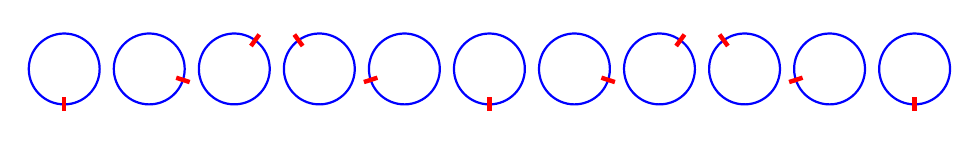
\begin{tikzpicture}[scale=0.9]

  \foreach \r in {0,...,10} {
      \begin{scope}[xshift={1.2*\r cm},  rotate=72*\r]
           {
  \draw[blue, thick] (0,0) circle(0.5); 
  \draw[ultra thick, red] (0,-0.4)--(0,-0.6);
}
       \end{scope}
    }

\end{tikzpicture}

 \caption{\label{fig:tau2n}The family of necklaces $\tau^{2n}$.}
\end{figure}

A first conclusion is that ${\mathop{\mathrm{Ker}}\nolimits} H_1 = \langle d(f) \rangle = \langle \tau^{2n} \rangle$.
And finally : 

$$\pi_1({\mathop{\mathrm{Conf}}\nolimits} \mathcal{L}_n)
\cong 
\pi_1({\mathop{\mathrm{Conf}}\nolimits} \mathcal{L}_n^*) / \langle \tau^{2n} \rangle
\cong
CB_n/\langle \zeta^{2n} \rangle$$
\end{proof}

Let us end the section with few remarks:

\begin{remark}
 Since $\zeta^n$ generates the center of $CB_n$ then the group generated  by  $\zeta^{2n}$ is normal: so we can effectively write $\langle \zeta^{2n} \rangle$
instead of  $\langle \langle \zeta^{2n} \rangle \rangle$; let us also recall that, denoting by $Mod_{n+2}(S^2)$  the mapping class group
of the $n+2$-punctured sphere,  $CB_n/\langle \zeta^{n} \rangle$ is isomorphic to the subgroup
of $Mod_{n+2}(S^2)$ fixing  two punctures (see \cite{CC}).
\end{remark}

\begin{remark} \label{rk:circular}
 In Theorem  \ref{th:circular}  we constructed a map $h_n: CB_n \to \pi_1({\mathop{\mathrm{Conf}}\nolimits} \mathcal{L}_n)$
where the generator $\zeta$ in $CB_n$ corresponds to  the move $\tau$ in $\pi_1({\mathop{\mathrm{Conf}}\nolimits} \mathcal{L}_n)$,
while   the generator $\sigma_i$ in $CB_n$ corresponds to the move $\sigma_i$ which permutes the $i$-th circle
with the $i+1$-th one (modulo $n$) by passing the $i$-th circle through the $i+1$-th. The kernel of $h_n$ 
is the group generated  by  $\zeta^{2n}$ and the group $\pi_1({\mathop{\mathrm{Conf}}\nolimits} \mathcal{L}_n)$ admits the following 
group presentation:

$$\pi_1({\mathop{\mathrm{Conf}}\nolimits} \mathcal{L}_n) = \left\langle \sigma_1,\ldots,\sigma_n, \tau \mid
\begin{array}{l}
\sigma_i\sigma_{i+1}\sigma_i = \sigma_{i+1}\sigma_i\sigma_{i+1} \quad \text{ for } i = 1,2\ldots, n, \\
\sigma_i\sigma_j=\sigma_j\sigma_i \quad \text{ for } |i-j| \neq 1, \\
{\bar{{\tau}}} \sigma_i \tau =\sigma_{i+1} \quad \text{ for } i = 1,2\ldots, n \\
\tau^{2n}=1
\end{array}
\right\rangle.
$$
\end{remark}

\section{Action on $\pi_1({\mathbb{R}}^3\setminus \mathcal{L}_n$)}
\label{sec:action}

 As recalled in the introduction, we denote:
 \begin{itemize}
 \item  the configuration space 
  of $n$ unlinked Euclidean circles  by $\mathcal{R}_n$ and $\pi_1(\mathcal{R}_n)$ by $R_n$;
\item  the configuration of $n$ unlinked Euclidean circles being all parallel to a fixed plane, say the $yz$-plane,
by $\mathcal{UR}_n$ and  its fundamental group by $WB_n$.
\end{itemize}

Clearly  $WB_n$ can be seen as a subgroup of $R_n$ and it is generated by two families of elements, $\rho_i$ and $\sigma_i$ 
(see figure \ref{fig:moves} and \cite{BH}):  $\rho_i$ is the path permuting the $i$-th and the $i+1$-th circles by passing over,
while $\sigma_i$ permutes them by passing the $i$-th circle through the $i+1$-th.

A {\emph{{motion}}} of a compact submanifold $N$ in a  manifold $M$ is a path $f_t$
in $\text{Homeo}_c(M)$ such that $f_0=\textup{id}$ and $f_1(N)=N$, where $\text{Homeo}_c(M)$
denotes  the group of homeomorphisms of $M$ with compact support. A
motion is called {\emph{{stationary}}} if $f_t(N)=N$ for all $t\in[0,1]$. The {\emph{{motion
group}}} $\mathcal{M}(M,N)$ of $N$ in $M$ is the group of equivalence classes of
motion of $N$ in $M$  where two motions $f_t,g_t$ are equivalent if
$(g^{-1}f)_t$ is homotopic relative to endpoints to a stationary motion.
The notion of motion groups was proposed by R.~Fox, and studied
by P.~Dahm, one of his students. The first published article on the topic is \cite{G1}.
Notice that motion groups generalize fundamental groups of configuration spaces,
and  that each motion is equivalent to a motion that fixes
a point $*\in M \setminus N$ , when $M$ is non-compact, it is possible to define a homomorphism
(the \emph{Dahm morphism}):
\begin{equation*}
D_N: \mathcal{M}(M,N)\to {\mathop{\mathrm{Aut}}\nolimits}(\pi_1(M \setminus N,*))
\end{equation*}
 sending an element represented by the motion $f_t$, into the automorphism
induced on $\pi_1(M\setminus N,*)$ by $f_1$.

When $M={\mathbb{R}}^3$ and $N$ is a set $\mathcal{L}'$ of $n$ unlinked Euclidean circles 
we get a map 
\begin{equation*}
D_{\mathcal{L}'}:R_n \to {\mathop{\mathrm{Aut}}\nolimits}(\pi_1({\mathbb{R}}^3 \setminus \mathcal{L}',*))
\end{equation*}
This map is injective (see \cite{G1}) and sends generators of $R_n$ (and therefore of $WB_n$) in 
 the following  automorphisms of the free group $F_n=\langle x_1, \ldots, x_n \rangle$: 
$$\sigma_i : 
\left\{\begin{array}{l}
x_i \mapsto x_{i} x_{i+1} {\bar{{x_{i}}}} \\
x_{i+1} \mapsto x_i \\
x_{j} \mapsto x_j \quad j \neq i,i+1\\     
\end{array}\right.
\; 
\rho_i : 
\left\{\begin{array}{l}
x_i \mapsto   x_{i+1}   \\
x_{i+1} \mapsto x_i \\
x_{j} \mapsto x_j \quad  j \neq i,i+1\\       
\end{array}\right.
$$
$$
\tau_j : 
\left\{\begin{array}{l}
x_j \mapsto   {\bar{{x_j}}}   \\
x_{k} \mapsto x_k \quad   k \neq j\\       
\end{array}\right.$$ 
where $i=1,\ldots, n-1$ and $j=1,\ldots, n$.
 
Now let  $\mathcal{L}_n$ be a necklace: by forgetting 
the core circle $K_0$ we obtain a map from ${\mathop{\mathrm{Conf}}\nolimits} \mathcal{L}_n$ to $\mathcal{R}_n$.
To  $\Gamma = \mathcal{L}_n(t)$ in $\pi_1({\mathop{\mathrm{Conf}}\nolimits} \mathcal{L}_n)$,
we can therefore associate an automorphism 
$D_{\mathcal{L}_n}(\Gamma) : \pi_1({\mathbb{R}}^3\setminus \mathcal{L}_n) 
\to \pi_1({\mathbb{R}}^3\setminus \mathcal{L}_n)$.   It is easy to  compute the $\pi_1$ of the complement of $\mathcal{L}_n$ by giving its Wirtinger presentation:
$$\pi_1({\mathbb{R}}^3 \setminus \mathcal{L}_n) = \left\langle x_1,\ldots,x_n,y \mid x_iy=yx_i, i=1\ldots,n \right\rangle$$
so that we obtain
$$\pi_1({\mathbb{R}}^3 \setminus \mathcal{L}_n) \cong F_n \times {\mathbb{Z}}.$$
The action of the generators of $\pi_1({\mathop{\mathrm{Conf}}\nolimits} \mathcal{L}_n)$ are (with indices  modulo $n$):
$$\sigma_i : 
\left\{\begin{array}{l}
x_i \mapsto x_{i} x_{i+1} {\bar{{x_{i}}}} \\
x_{i+1} \mapsto x_i \\
x_{j} \mapsto x_j \quad j \neq i,i+1\\
y \mapsto y         
\end{array}\right.
\qquad 
\tau : 
\left\{\begin{array}{l}
x_j \mapsto x_{j+1} \\
y \mapsto y         
\end{array}\right.$$

\begin{lemma}
\label{lem:dahm}

\begin{enumerate}
\item Let  $D_{\mathcal{L}_n} : \pi_1({\mathop{\mathrm{Conf}}\nolimits} \mathcal{L}_n) \to {\mathop{\mathrm{Aut}}\nolimits}  \pi_1({\mathbb{R}}^3\setminus \mathcal{L}_n)$
be  the  Dahm morphism;
then ${\mathop{\mathrm{Ker}}\nolimits} D_{\mathcal{L}_n} = \langle \tau^n \rangle = {\mathbb{Z}} / 2{\mathbb{Z}}$.
\item Let $\Phi$ be the natural map $\Phi : \pi_1({\mathop{\mathrm{Conf}}\nolimits} \mathcal{L}_n) \to  R_n$ 
induced by forgetting the core circle $K_0$. Then ${\mathop{\mathrm{Ker}}\nolimits} \Phi = \langle \tau^n \rangle = {\mathbb{Z}}/ 2{\mathbb{Z}}$.
\end{enumerate}
\end{lemma}

\begin{proof}
We first notice some facts:

(a) The following diagram is commutative :
$$ \xymatrix{
{}\pi_1({\mathop{\mathrm{Conf}}\nolimits} \mathcal{L}_n) \ar[r]^-{D_{\mathcal{L}_n}}\ar[d]_-{\Phi}  & {\mathop{\mathrm{Aut}}\nolimits}  \pi_1({\mathbb{R}}^3\setminus \mathcal{L}_n) \ar[d]^-{\Psi} \\
  R_n \ar[r]_-{D_{\mathcal{L}'_n}}        &  {\mathop{\mathrm{Aut}}\nolimits}  \pi_1({\mathbb{R}}^3\setminus \mathcal{L}'_n)
}
$$
where $\Phi$ and $\Psi$ are natural maps induced by the inclusion $\mathcal{L}'_n \subset \mathcal{L}_n$.
Remark that  $\Psi$ is then the  map which forgets the generator $y$ in $ \pi_1({\mathbb{R}}^3\setminus \mathcal{L}_n)$ and therefore 
$$\psi(D_{\mathcal{L}_n})(\sigma_i) : 
\left\{\begin{array}{l}
x_i \mapsto x_{i} x_{i+1} {\bar{{x_{i}}}} \\
x_{i+1} \mapsto x_i \\
x_{j} \mapsto x_j \quad j \neq i,i+1       
\end{array}\right.
\qquad 
\psi(D_{\mathcal{L}_n})(\tau) : 
\left\{\begin{array}{l}
x_j \mapsto x_{j+1}        
\end{array}\right.$$
where indices are modulo $n$.
Comparing with Theorem \ref{thmCB} and \ref{th:circular} we deduce that the $ \Psi \circ D_{\mathcal{L}_n} \circ h_n = \rho_{CB}$
and  ${\mathop{\mathrm{Ker}}\nolimits} \Psi \circ D_{\mathcal{L}_n} \circ h_n = \langle \zeta^n \rangle$.

(b) As we already recall, it is known that for the trivial link $\mathcal{L}'_n$ 
the Dahm morphism $D_{\mathcal{L}'_n}$ is injective (\cite{G1})
(where $h_n : CB_n \to \pi_1({\mathop{\mathrm{Conf}}\nolimits} \mathcal{L}_n)$ is induced by \ref{th:circular}).

(c) $\Psi$ is  injective when restricted to the image of $D_{\mathcal{L}_n}$.
If $\Psi(f)={\mathop{\mathrm{id}}\nolimits}$, then $f(x_i)=x_i$ for all $i=1,\ldots,n$.
If $f \in {\mathop{\mathrm{Im}}\nolimits} D_{\mathcal{L}_n}$, then due to the action of the generators ($\sigma_i$ and $\tau$), it implies $f(y)=y$.
Finally if $\Psi(f)={\mathop{\mathrm{id}}\nolimits}$ and $f \in {\mathop{\mathrm{Im}}\nolimits} D_{\mathcal{L}_n}$, then $f={\mathop{\mathrm{id}}\nolimits}$. Then ${\mathop{\mathrm{Ker}}\nolimits} D_{\mathcal{L}_n} \circ h_n = \langle \zeta^n \rangle$.
Clearly, $ \tau^n \in {\mathop{\mathrm{Ker}}\nolimits} D_{\mathcal{L}_n} $; on the other hand 
since $h_n$ is surjective, if $x \in {\mathop{\mathrm{Ker}}\nolimits} D_{\mathcal{L}_n} $, 
then $x\in {\mathop{\mathrm{Im}}\nolimits} (\langle \zeta^n \rangle)$ and therefore $x \in \langle \tau^n \rangle$
(see Remark \ref{rk:circular}).

\bigskip

For the second statement it is therefore enough to prove that the kernel of 
$D_{\mathcal{L}_n}$ coincides with  the kernel of $\Phi$.
$$
\begin{array}{rcll}
\gamma \in {\mathop{\mathrm{Ker}}\nolimits} \Phi 
& \iff & \Phi(\gamma)= {\mathop{\mathrm{id}}\nolimits} \\
& \iff & D_{\mathcal{L}'_n} \circ \Phi (\gamma) = {\mathop{\mathrm{id}}\nolimits} &\qquad \text{because $D_{\mathcal{L}'_n}$ is injective} \\
& \iff & \Psi \circ D_{\mathcal{L}_n}(\gamma) = {\mathop{\mathrm{id}}\nolimits} &\qquad \text{because the diagram commutes} \\
& \iff & D_{\mathcal{L}_n}(\gamma) = {\mathop{\mathrm{id}}\nolimits} &\qquad \text{because $\Psi_{| D_{\mathcal{L}_n}}$  is injective}\\
& \iff & \gamma \in {\mathop{\mathrm{Ker}}\nolimits}  D_{\mathcal{L}_n}(\gamma)&\\
\end{array}
$$

\end{proof}

\section{Characterization of automorphisms}
\label{sec:auto}

We will use the following notation: for a word ${\bar{{w}}}= w^{-1}$, 
for an automorphism ${\bar{{\alpha}}}=\alpha^{-1}$.
A famous result of Artin, characterizes automorphisms induced by braids.
\begin{theorem}[Artin]
The automorphisms induced by the action of $B_n$ on $F_n$ are exactly 
the automorphisms $\phi$ of ${\mathop{\mathrm{Aut}}\nolimits} F_n$ that verify the two conditions below:
\begin{equation}
\label{eq:artinconj1}
\phi(x_i)=w_i x_{\pi(i)} {\bar{{w_i}}}  
\end{equation}
for some $w_1,\ldots,w_n \in F_n$ and some permutation $\pi \in \mathcal{S}_n$, and:
\begin{equation}
\label{eq:artinconj2}
\phi(x_1x_2\cdots x_n) = x_1x_2\cdots x_n
\end{equation}
\end{theorem}

\bigskip

Interestingly, if we do not require condition (\ref{eq:artinconj2}), we recover 
exactly automorphisms of ${\mathop{\mathrm{Aut}}\nolimits} F_n$ induced by welded braids. Recall 
that the welded braid group is generated by two types of moves $\sigma_i, \rho_i$, which induced 
two kinds of automorphisms also denoted $\sigma_i, \rho_i$ and described in section \ref{sec:action}.

\begin{theorem}[Theorem 4.1 of \cite{FRR}]
The automorphisms of ${\mathop{\mathrm{Aut}}\nolimits} F_n$ induced  by the action of $WB_n$ on $F_n$ are exactly  those verifying (\ref{eq:artinconj1}).
\end{theorem}

 As a straightforward consequence we have
 that the natural map $B_n \to WB_n$
sending $\sigma_i$ into $\sigma_i$ is injective. We will show in  section \ref{ssec:linearnecklace} a geometric interpretation of
such an embedding.
 
\bigskip

Now we relax condition (\ref{eq:artinconj2}) and characterize automorphisms induced by our configurations.
\begin{theorem}
\label{th:circularartin}
The automorphisms induced by the action 
$\pi_1({\mathop{\mathrm{Conf}}\nolimits} \mathcal{L}_n)$ on ${\mathop{\mathrm{Aut}}\nolimits} F_n$ are exactly 
the automorphisms $\phi$ of ${\mathop{\mathrm{Aut}}\nolimits} F_n$ that verify the two conditions below:
\begin{equation}
\label{eq:conj1}
\phi(x_i)=w_i x_{\pi(i)} {\bar{{w_i}}}  
\end{equation}
for some $w_1,\ldots,w_n \in F_n$ and some permutation $\pi \in \mathcal{S}_n$, and:
\begin{equation}
\label{eq:conj2}
\phi(x_1x_2\cdots x_n) = w  x_1x_2\cdots x_n {\bar{{w}}} 
\end{equation}
for some $w \in F_n$.
\end{theorem}

\begin{proof}
Notations:
\begin{itemize}
  \item We denote by $\mathcal{A}_n$ the set of automorphisms of ${\mathop{\mathrm{Aut}}\nolimits} F_n$ induced
by $\pi_1({\mathop{\mathrm{Conf}}\nolimits} \mathcal{L}_n)$ and $\mathcal{B}_n$ the set of automorphisms of ${\mathop{\mathrm{Aut}}\nolimits} F_n$
that verify conditions (\ref{eq:conj1}) and (\ref{eq:conj2}).
We will prove $\mathcal{A}_n=\mathcal{B}_n$.

  \item We set $\Delta = x_1x_2\cdots x_n$.

  \item And for any $w\in F_n$, we set the automorphism
$g_w \in {\mathop{\mathrm{Aut}}\nolimits} F_n$ defined by $g_w(x_i) = w x_i {\bar{{w}}}$.
For any $w'\in F_n$, we have $g_w(w')= w w' {\bar{{w}}}$.
\end{itemize}

 
\bigskip

First of all, the action of $\pi_1({\mathop{\mathrm{Conf}}\nolimits} \mathcal{L}_n)$ on ${\mathop{\mathrm{Aut}}\nolimits} F_n$
is generated by the automorphisms $\sigma_i$ ($i=1,\ldots,n$) and $\tau$
that verify equations (\ref{eq:conj1}) and (\ref{eq:conj2}). 
In fact for $i=1,\ldots,n-1$, $\sigma_i(\Delta)=\Delta$ ; 
$\sigma_n(\Delta) =x_n {\bar{{x_1}}} \Delta x_1 {\bar{{x_n}}}$, $\tau(\Delta)={\bar{{x_1}}} \Delta x_1$.
It proves $\mathcal{A}_n \subset \mathcal{B}_n$.

\bigskip

The remaining part is to prove $\mathcal{B}_n \subset \mathcal{A}_n$: given an automorphism $f \in {\mathop{\mathrm{Aut}}\nolimits} F_n$ that verifies
conditions (\ref{eq:conj1}) and (\ref{eq:conj2}), we express it as the automorphism induced by
some element of $\pi_1({\mathop{\mathrm{Conf}}\nolimits} \mathcal{L}_n)$. 
 
\bigskip

\textbf{1st step. Generation of $g_{x_1}$.}

A simple verification prove the following equation: the automorphism $g_{x_1}$ 
defined by $x_i \mapsto x_1 x_i {\bar{{x_1}}}$ is generated by
elements of $\mathcal{A}_n$.
$$g_{x_1} = \sigma_1 \circ \sigma_2 \circ \cdots \circ \sigma_{n-1} \circ {\bar{{\tau}}}$$

\bigskip

\textbf{2nd step. Generation of $g_{x_k}$.}

$g_{x_k} \in \mathcal{A}_n$ by the following relation:
$$g_{x_k} = \underbrace{\tau\circ \tau \circ \cdots \tau}_{k-1 \text{ occurrences}} \circ g_{x_1} \circ 
\underbrace{{\bar{{\tau}}}\circ{\bar{{\tau}}} \circ \cdots {\bar{{\tau}}}}_{k-1 \text{ occurrences}}$$
We also generate $g_{x_k^{-1}}$ as the inverse of $g_{x_k}$.

\bigskip

\textbf{3rd step. Generation of $g_w$.}

Let $w \in F_n$. We generate the automorphism $g_w$ by induction on the length of $w$.
Suppose that $w = x_k w'$ with $w' \in F_n$ of length strictly less than the length of $w$.
Suppose that $g_{w'} \in  \mathcal{A}_n$. Then
$$g_w = g_{x_k} \circ g_{w'} \in \mathcal{A}_n.$$

\bigskip

\textbf{4th step. Simplification of the action on $\Delta$.}

Let $f\in {\mathop{\mathrm{Aut}}\nolimits} F_n$. Suppose that $f$ verifies conditions (\ref{eq:conj1}) and (\ref{eq:conj2}).
In particular, let $w \in F_n$ such that $f(\Delta)= w \Delta {\bar{{w}}}$.
Then $g_{{\bar{{w}}}} \circ f$ still satisfies conditions of type (\ref{eq:conj1})
and the condition (\ref{eq:artinconj2}):  $g_{{\bar{{w}}}} \circ f(\Delta)=\Delta$.

\bigskip

\textbf{5th step. Artin's theorem.}

Therefore we can suppose that, given $f \in \mathcal{B}_n$ and after a composition $g \in \mathcal{A}_n$ of elements $\sigma_i$, $\tau$, 
$g \circ f$ verifies condition (\ref{eq:artinconj1}) (which is exactly condition (\ref{eq:conj1})) and condition (\ref{eq:artinconj2}).
By Artin's theorem $g\circ f \in \mathcal{A}_n$. Hence $f \in \mathcal{A}_n$.
It ends the proof of $\mathcal{B}_n \subset \mathcal{A}_n$, so that we get 
$\mathcal{A}_n=\mathcal{B}_n$.

\end{proof}

\section{Zero angular sum}
\label{sec:zero}

We say that $\Gamma \in \pi_1({\mathop{\mathrm{Conf}}\nolimits} \mathcal{L}_n)$
has {\emph{{zero angular sum}}} if $\Gamma \in \langle \sigma_1,\ldots,\sigma_n\rangle$.
This definition is motivated by the fact that a move $\sigma_i$
shifts the component $K_i$ by an angle of --say-- $+\frac{2\pi}{n}$
while $K_{i+1}$ is shifted by $-\frac{2\pi}{n}$, the sum of these angles being zero.
On the other hand $\tau$, moves each $K_i$ by an angle of --say-- $+\frac{2\pi}{n}$,
with a sum of $2\pi$.
The aim of this section is to characterize the zero angular sum condition 
at the level of automorphisms. We will define a kind of total winding number 
$\epsilon(\Gamma)$ about the axis of rotation of $K_0$.

Let $\epsilon : \pi_1({\mathop{\mathrm{Conf}}\nolimits} \mathcal{L}_n) \to {\mathbb{Z}}$
defined as follows: to $\Gamma \in \pi_1({\mathop{\mathrm{Conf}}\nolimits} \mathcal{L}_n)$,
we associate an automorphism $\phi = D_{\mathcal{L}_n}(\Gamma)$
by the Dahm morphism.
By theorem \ref{th:circularartin}, $\phi(x_1x_2\cdots x_n) = w  x_1x_2\cdots x_n {\bar{{w}}}$,
for some $w \in F_n$. We define $\epsilon(\Gamma) = \ell({\bar{{w}}}) \in {\mathbb{Z}}$
to be the algebraic length of the word ${\bar{{w}}}$. 
We have the following characterization of zero angular sum:
\begin{proposition}
\label{prop:angmom}
$\Gamma \in \langle \sigma_1,\ldots,\sigma_n\rangle$
if and only if $\epsilon(\Gamma) = 0$.
\end{proposition}

\begin{proof}
We have the following facts:
\begin{itemize}
  \item $\epsilon$ is a morphism.
  \item If we denote $\Delta = x_1\cdots x_n$ then for
 $i=1,\ldots,n-1$, $\sigma_i(\Delta)=\Delta$; 
$\sigma_n(\Delta) =x_n {\bar{{x_1}}} \Delta x_1 {\bar{{x_n}}}$, $\tau(\Delta)={\bar{{x_1}}} \Delta x_1$.
It implies $\epsilon(\sigma_i)=0$ and $\epsilon(\tau)=1$.

  \item Any $\Gamma \in  \pi_1({\mathop{\mathrm{Conf}}\nolimits} \mathcal{L}_n)$ can be written
$\Gamma = \tau^k \sigma_{i_1}\cdots \sigma_{i_\ell}$ (by using the relations 
$\sigma_i \tau = \tau\sigma_{i+1}$).
  
  \item Hence  $\epsilon(\Gamma)=0$ implies  $k=0$, in which case
 $\Gamma \in  \langle \sigma_1,\ldots,\sigma_n\rangle$.
\end{itemize}

\end{proof}

We recall that the {\emph{{affine braid group}}}  $\tilde{A}_{n-1}$, is the group obtained by the group presentation of   $B_{n+1}$ 
 by replacing the relation $\sigma_{n} \sigma _1 =\sigma _1\sigma_{n}$ with the relation $\sigma_{n} \sigma _1\sigma_{n} =\sigma _1\sigma_{n} \sigma _1$.
By comparison of group presentations one deduces that   $CB_n = \tilde{A}_{n-1} \rtimes \langle\zeta\rangle$ (see also \cite{CC,KP}).  It then follows from Theorem \ref{th:circular}
and Remark  \ref{rk:circular} that  $\pi_1({\mathop{\mathrm{Conf}}\nolimits} \mathcal{L}_n)= \tilde{A}_{n-1} \rtimes \langle\tau\rangle$.  Since $\tau$ has finite order, $\pi_1({\mathop{\mathrm{Conf}}\nolimits} \mathcal{L}_n)$
inherits some properties of  $\tilde{A}_{n-1}$, in particular:

\begin{corollary}
The group $\pi_1({\mathop{\mathrm{Conf}}\nolimits} \mathcal{L}_n)$ is linear and, provided with the group presentation given in Remark \ref{rk:circular}, has solvable word problem.
\end{corollary}

On the other hand, it follows from Theorem \ref{th:circular} and Proposition \ref{prop:angmom} that:

 
 
 \begin{proposition}
 The affine braid group on $n$ strands, $\tilde{A}_{n-1}$ is isomorphic to  the subgroup of  $\pi_1({\mathop{\mathrm{Conf}}\nolimits} \mathcal{L}_n)$
 consisting of elements of zero angular sum.
 \end{proposition}
 
 
 
Consider now the representation $\rho_{\mathop{\mathrm{Aff}}\nolimits} :  \tilde{A}_{n-1} \longrightarrow {\mathop{\mathrm{Aut}}\nolimits} F_n$ 
induced by the action of $\pi_1({\mathop{\mathrm{Conf}}\nolimits} \mathcal{L}_n)$ on ${\mathop{\mathrm{Aut}}\nolimits} F_n$ (obtained by setting $y=1$).
 
 
 
 $$ i\not=n:
\rho_{\mathop{\mathrm{Aff}}\nolimits} (\sigma_{i}) : \left\{
\begin{array}{ll}
x_{i} \longmapsto x_{i} \, x_{i+1} \, {\bar{{x_i}}}, &  \\ 
x_{i+1} \longmapsto x_{i}, & \\ 
x_{j} \longmapsto x_{j}, &  j\neq i,i+1.
\end{array} \right.
$$
$$
\rho_{\mathop{\mathrm{Aff}}\nolimits} (\sigma_{n}) : 
\left\{
\begin{array}{ll}
x_{1} \longmapsto  x_{n}  &  \\
x_{n} \longmapsto
x_{n} x_{1}  {\bar{{x_{n}}}} , & \\ 
x_{j} \longmapsto x_{j}, &  j\neq 1, n.
\end{array} \right.
$$

\begin{theorem}\label{thm:affine}

\begin{enumerate}[i)]
\item The representation  $\rho_{\mathop{\mathrm{Aff}}\nolimits} :  \tilde{A}_{n-1} \longrightarrow {\mathop{\mathrm{Aut}}\nolimits} F_n$  is faithful. 
\item An element $\phi \in Aut F_n$ belongs to $\rho_{\mathop{\mathrm{Aff}}\nolimits} (\tilde{A}_{n-1})$ if and only if it verifies the conditions below:
\begin{equation}
\label{eq:conj1bis}
\phi(x_i)=w_i x_{\pi(i)} {\bar{{w_i}}}  
\end{equation}
for some $w_1,\ldots,w_n \in F_n$ and some permutation $\pi \in \mathcal{S}_n$, and:
\begin{equation}
\label{eq:conj2bis}
\phi(x_1x_2\cdots x_n) = w  x_1x_2\cdots x_n {\bar{{w}}} 
\end{equation}
for some $w \in F_n$ with algebraic length $\ell(w)=0$.
\end{enumerate}
 \end{theorem}

\begin{proof}
The kernel of $\rho_{\mathop{\mathrm{Aff}}\nolimits} $ is a subgroup of the kernel of $\Psi \circ D_{\mathcal{L}_n} \circ h_n$, which is generated by $\tau^n$ (Lemma \ref{lem:dahm}).
Since $\tau^n$ generates the center of $\pi_1({\mathop{\mathrm{Conf}}\nolimits} \mathcal{L}_n)$, the kernel of  $\rho_{\mathop{\mathrm{Aff}}\nolimits} $ is a subgroup of the center of  $\tilde{A}_{n-1}$.
Since the center of $\tilde{A}_{n-1} $ is trivial (see for instance \cite{JA}) we can conclude that $\rho_{\mathop{\mathrm{Aff}}\nolimits}$ is faithful. The characterization given in the second statement follows 
 combining Theorem \ref{th:circularartin} and Proposition \ref{prop:angmom}.
\end{proof}

\section{The linear necklace}
\label{ssec:linearnecklace}

Let $\mathcal{C}^*_n =  K_1 \cup\ldots\cup K_n$ be the link where
each $K_i$ is a Euclidean circle  parallel to the $yz$-plane and centered at the $x$-axis.
We call such a  link a {\emph{{linear necklace}}}, thinking of the $x$-axis as $K_0$, a circle
passing through a point at infinity.
\begin{figure}
 
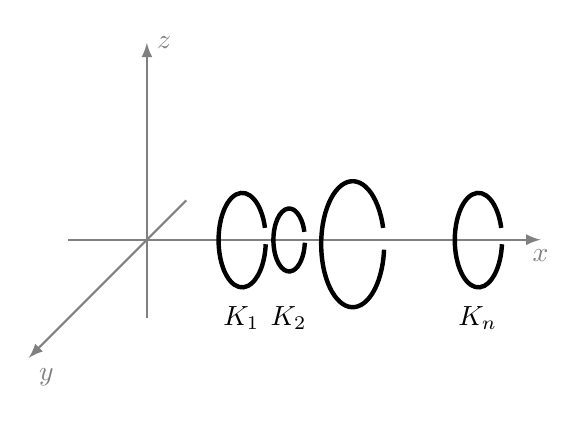
\begin{tikzpicture}[scale=1]

\begin{scope}

\draw[->,>=latex,gray,thick] (-1,0)--(5,0) node[below]{$x$};
\draw[->,>=latex,gray,thick] (0,-1)--(0,2.5) node[right]{$z$};
\draw[->,>=latex,gray,thick] (0.5,0.5)--(-1.5,-1.5) node[below right]{$y$};

\draw[ultra thick] (1.5,0.15) arc (15:355:0.3 and 0.6);
\draw[ultra thick] (2,0.1) arc (15:355:0.2 and 0.4);
\draw[ultra thick] (3,0.15) arc (15:355:0.4 and 0.8);
\draw[ultra thick] (4.5,0.15) arc (15:355:0.3 and 0.6);
 \node at (1.2,-1) {$K_1$}; 
 \node at (1.8,-1) {$K_2$}; 
 \node at (4.2,-1) {$K_n$}; 
\end{scope}

\end{tikzpicture}

 \caption{A linear necklace. \label{fig:linearnecklace}}
\end{figure}

We recall that $\mathcal{UR}_n$ is the configuration space  of $n$ 
disjoint Euclidean circles lying on planes parallel to the $yz$-plane.
We have that:
\begin{theorem}
The inclusion of  ${\mathop{\mathrm{Conf}}\nolimits} \mathcal{C}^*_n$ into $\mathcal{UR}_n$ induces an injection at the level 
of fundamental groups.
\end{theorem}
\begin{proof}
Let us remark that the moves $\sigma_1, \ldots, \sigma_{n-1}$ depicted in figure 2 belong to $\pi_1({\mathop{\mathrm{Conf}}\nolimits} \mathcal{C}^*_n) $. Actually, they
generate $\pi_1({\mathop{\mathrm{Conf}}\nolimits} \mathcal{C}^*_n) $; in fact, the position of any circle $K_i$ of $\mathcal{C}^*_n$
is determined by the intersection with the half-plane $y=0$ and $z>0$.
It follows that the configuration space of linear necklaces, ${\mathop{\mathrm{Conf}}\nolimits} \mathcal{C}^*_n$, 
can be identified with the configuration space of $n$ distinct points in the (half-)plane, 
so that $\pi_1({\mathop{\mathrm{Conf}}\nolimits} \mathcal{C}^*_n) =B_n$,  where  generators are  exactly moves $\sigma_1, \ldots, \sigma_{n-1}$.
\end{proof}

The previous result provides then a geometrical interpretation for the algebraic embedding of 
$B_n$ into $WB_n$ as subgroups of ${\mathop{\mathrm{Aut}}\nolimits}(F_n)$.

\subsection*{Pure subgroups.}

Let us denote by ${\mathop{\mathrm{Conf}}\nolimits}_{\text{Ord}}\mathcal{C}_n$ the configuration space of $n$ 
disjoint Euclidean  ordered circles lying on planes parallel to the $yz$-plane:
 $\pi_1({\mathop{\mathrm{Conf}}\nolimits}_{\text{Ord}} \mathcal{C}_n)$ is called the {\emph{{pure welded  braid group}}} on $n$ strands and will be denoted by $WP_n$,
 while $\pi_1({\mathop{\mathrm{Conf}}\nolimits}_{\text{Ord}} \mathcal{C}^*_n)$ is isomorphic to the pure braid group $P_n$.  Previous results imply that $P_n$ embeds geometrically in 
 $WP_n$.
 
More precisely, the group  $\pi_1({\mathop{\mathrm{Conf}}\nolimits}_{\text{Ord}} \mathcal{C}^*_n)$  is generated 
 by the family of paths $\lambda_{i,j}$ for $1{\leqslant} i < j {\leqslant} n$:  $\lambda_{i,j}$ moves 
 only the $i$-th circle that  passes inside  the following ones until the $j-1$-th one, 
  inside-outside the  $j$-th one and that  finally comes back passing inside the other circles.
 
Notice also that  in \cite{BH} was introduced the configuration spaces of circles lying on parallel planes of different size, that 
 we can denote by $\mathcal{UR}^<_n$.  We can take as base-point for $\pi_1(\mathcal{UR}^<_n)$  a configuration
  of parallel circles with center on the $z$-axis and such that for any $i=1, \ldots, n-1$
 the $i$-th circle has radius greater than the radius of the $i+1$-th one. Let us remark that all other choices of base point  give conjugated subgroups  in  $WP_n$
 corresponding to different  permutations of circles.   As shown in \cite{BH},  $\pi_1(\mathcal{UR}^<_n)$ is generated by $\delta_{i,j}$ for $1{\leqslant} i < j {\leqslant} n$:  $\delta_{i,j}$ moves only the $i$-th circle that 
  passes outside  the $j-1$-th one (without passing inside-outside the other circles) and moves back (without passing inside-outside the other circles). 
  
 Let us recall that $\pi_1(\mathcal{UR}^<_n)$ is  called {\emph{{upper McCool group}}}
 in \cite{CPVW} and denoted by $P\Sigma_n^+$:   it is interesting to remark  that $P\Sigma_n^+$ and $P_n$ have isomorphic Lie algebras associated to the lower central series
  and the groups themselves are isomorphic for $n=2,3$ (\cite{CPVW}). A.~Suciu communicated to  us that using ideas from \cite{CoS}  it is possible to show that
  the ranks  of \emph{Chen groups} are different for $n>3$ and therefore $P\Sigma_n^+$ and $P_n$ are not isomorphic for 
 $n>3$.

\section*{Appendix: proof of Theorem \ref{thmCB}}
\begin{theorem1} 
The kernel of $\rho_{CB}:  CB_n \to {\mathop{\mathrm{Aut}}\nolimits} F_n$ is the cyclic group generated by $\zeta^n$.
\end{theorem1}

\begin{itemize}
  \item 
  Let us recall that when we restrict the map $D_{\mathcal{L}'}:R_n \to {\mathop{\mathrm{Aut}}\nolimits}(\pi_1({\mathbb{R}}^3 \setminus \mathcal{L}',*))$ to the braid group $B_n$
we get the usual Artin representation $\rho_A : B_n \to {\mathop{\mathrm{Aut}}\nolimits} F_n$:
$$\rho_A(\sigma_i) : 
\left\{\begin{array}{l}
x_i \mapsto x_{i} x_{i+1} {\bar{{x_{i}}}} \\
x_{i+1} \mapsto x_i \\
x_{j} \mapsto x_j \quad j \neq i,i+1\\    
\end{array}\right.
$$
for  the usual generators $\sigma_1, \ldots, \sigma_{n-1}$  of $B_n$.

Therefore we can define the group   $B_n \ltimes_{\rho_A} F_n$:
as generators  we will  denoted by $\alpha_1, \ldots, \alpha_{n-1}$ the generators of the factor
$B_n$ and  by $\eta_1,\ldots \eta_n$ a set  of generators for $F_n$.
According to such a set of generators a possible complete set of relations is the following:
$$
\begin{array}{l}
\alpha_i\alpha_{i+1}\alpha_i = \alpha_{i+1}\alpha_i\alpha_{i+1} \quad \text{ for } i = 1,2\ldots, n-1, \\
\alpha_i\alpha_j=\alpha_j\alpha_i \quad \text{ for } |i-j| \neq 1, \\
\alpha_i^{-1} \eta_i \alpha_i =\eta_{i}\eta_{i+1}\eta_{i}^{-1} \quad \text{ for } i = 1,2\ldots, n-1 \\
\alpha_i^{-1} \eta_{i+1} \alpha_i =\eta_{i} \quad \text{ for } i = 1,2\ldots, n-1 \\
\alpha_i^{-1} \eta_k \alpha_i =\eta_{k}  \quad \text{ for } i = 1,2\ldots, n-1 \quad \text{ and }  k \not= i, i+1
\end{array}
$$

\item The group $CB_n$ is isomorphic to $B_n \ltimes_{\rho_A} F_n$ (\cite{CrP});
we left to the reader the verification that a possible isomorphism is the map
$\Theta_n : CB_n \to B_n \ltimes_{\rho_A} F_n$  defined as follows:
$\Theta_n(\zeta)=\sigma_{n-1} \cdots \sigma_1 \eta_1$, $\Theta_n(\sigma_j)=\alpha_j$ for $j=1, \ldots, n-1$
and $\Theta_n(\sigma_n)= \eta_1^{-1} \sigma_1^{-1} \cdots \sigma_{n-2}^{-1}  \sigma_{n-1} \sigma_{n-2} \cdots \sigma_1 \eta_1$.

Using the action by conjugation of $F_n$ on itself we get 
a representation $\chi_n: B_n \ltimes_{\rho_A} F_n \to {\mathop{\mathrm{Aut}}\nolimits} F_n$. More precisely,
$\chi_n(\alpha_j)=\rho_A(\sigma_j)$ and $\chi_n(\eta_i)(x_k)= x_i^{-1} x_k x_i$
for any $j=1,\ldots, n-1$ and $i,k=1,\ldots, n$.

\item One can easily verify on the images of generators that the composed homomorphism $\chi_n \circ \Theta_n: CB_n  \to {\mathop{\mathrm{Aut}}\nolimits} F_n$
coincides with $\rho_{CB} : CB_n  \to {\mathop{\mathrm{Aut}}\nolimits} F_n$ defined in Section \ref{sec:necklace}.   We claim  that the kernel of $\chi_n$ 
is generated by $\Theta(\zeta^n)$: since $\Theta_n$ is an isomorphism, then the kernel of $\rho_{CB}$ is generated by $\zeta^n$.

To prove that,  remark that the group generated by $\Theta(\zeta^n)$ is in the kernel of $\chi_n$ ;  let $w \in {\mathop{\mathrm{Ker}}\nolimits} \chi_n$
and write $w$ in the form $w=\alpha  \, \eta$ where $\alpha$ is written in the generators $\alpha_i$'s  and $\eta$ in the generators
$\eta_j$'s.   

Since $\chi_n(w)(x_j)=x_j$ for all generators $x_1, \ldots, x_n$ of $F_n$,
we have that $\chi_n(\alpha)(x_j)=\eta^{-1}(x_j)$, where  $\chi_n(\alpha)(x_j)= \rho_A(\alpha)(x_j)$,
identifying any usual braid generator $\sigma_i$ with corresponding $\alpha_i$.

It follows that $\rho_A(\alpha)$ is an inner automorphism, therefore $\alpha$ belongs
to the center of $B_n$ (see for instance \cite{BB}, Remark 1): more precisely
$\alpha=((\alpha_{n-1} \cdots \alpha_1)^n)^m$ for some  $m \in {\mathbb{Z}}$ and 
$\rho_A(\alpha)(x_j)=(x_1 \cdots x_n)^m x_j (x_1 \cdots x_n)^{-m}$. Then we can deduce 
that $\eta=(\eta_1 \cdots \eta_n)^m$ and $w= ((\alpha_{n-1} \cdots \alpha_1)^n)^m (\eta_1 \cdots \eta_n)^m$.
Using the defining relations
of $B_n \ltimes_{\rho_A} F_n$ we obtain that $w=(((\alpha_{n-1} \cdots \alpha_1) \eta_1)^n)^m$
$=\Theta(\zeta^n)^m$.

  
  
\end{itemize}
 
\section*{Acknowledgments}

The authors thank the referee of a previous version for his comments and Juan Gonz\'alez-Meneses for useful
discussions on representations of affine braid groups in terms of automorphisms. 
The authors are deeply indebted to  Martin Palmer for fruitful conversations on configurations spaces.
The research of the first author was partially supported by the French grant ANR-11-JS01-002-01 "VASKHO".
The research of the second  author was partially supported by the French grant ANR-12-JS01-002-01 "SUSI".

\begin{thebibliography}{99}

\bibitem{JA}
M.~A.~Albar and G.~L.~Johnson, 
\emph{The centre of the circular braid group.} 
Math. Japonica 30 (1985) 641--645.

\bibitem{ABMW} B. Audoux, P. Bellingeri, J.-B. Meilhan, E. Wagner,  
\emph{Homotopy classification of ribbon tubes and welded string links.} 
Preprint, arXiv:1407.0184.
  
  
\bibitem{BB} V. Bardakov and P. Bellingeri, 
\emph{On representations of Artin-Tits and surface braid groups.} 
J. Group Theory 14 (2011) 143--163. 

 

\bibitem{BP} B. Berceanu, S. Papadima, 
\emph{Universal representations of braid and braid-permutation groups.}
J. Knot Theory Ramifications 18 (2009) 999--1019.

\bibitem{BH} T. Brendle, A. Hatcher, 
\emph{Configuration spaces of rings and wickets.}
Comment. Math. Helv. 88 (2013) 131--162.

\bibitem{CaPa} F. Cantero, M. Palmer,
\emph{On  homological  stability  for  configuration
spaces  on  closed  background  manifolds.}
Preprint, arXiv:1406.4916.

\bibitem{CC} R. Charney, J. Crisp,
\emph{Automorphism groups of some affine and finite type Artin groups.}
Math. Res. Lett. 12 (2005) 321--333.

\bibitem{CP} R. Charney, D. Peifer, 
\emph{The $K(\pi,1)$ conjecture for affine braid groups.}
Comment. Math. Helv. 78 (2003) 584--600.

\bibitem{CoS} D. C.  Cohen, A. I.  Suciu, 
\emph{The Chen groups of the pure braid group.}
The \v{C}ech centennial (Boston, MA, 1993), 45--64, Contemp. Math., 181,
Amer. Math. Soc., Providence, RI, 1995.

\bibitem{CPVW} F. R. Cohen, J. Pakianathan, V. V. Vershinin, J. Wu, 
\emph{Basis-conjugating automorphisms of a free group and associated Lie algebras.}
Groups, homotopy and configuration spaces, 147--168, Geom. Topol. Monogr., 13, Geom. Topol. Publ., Coventry, 2008.

\bibitem{CrP}
J.~Crisp and L.~Paris,
\emph{Artin groups of type B and D.} 
Adv. Geom. 5 (2005), 607--636.

\bibitem{FRR} R. Fenn, R. Rim\'anyi, C. Rourke, 
\emph{The braid-permutation group.}
Topology 36 (1997) 123--135.

\bibitem{FS} M. Freedman, R. Skora, 
\emph{Strange actions of groups on spheres.}
J. Differential Geom. 25 (1987) 75--98.

\bibitem{G1} D. Goldsmith,
\emph{The theory of motion groups.}
Michigan Math. J. 28 (1981) 3--17.

\bibitem{G2} D. Goldsmith,
\emph{Motion of links in the 3-sphere.}
Math. Scand. 50 (1982) 167--205.

\bibitem{Hu} M. Hutchings,
\emph{Introduction to higher homotopy groups and obstruction theory.}
\href{https://math.berkeley.edu/~hutching/teach/215b-2011/homotopy.pdf}{Link to personal web page.}

\bibitem{KP} R. Kent, D. Peifer,
\emph{A geometric and algebraic description of annular braid groups.}
Internat. J. Algebra Comput. 12 (2002) 85--97. 

\end{thebibliography} 

\bigskip
\bigskip

\end{document}
